\documentclass{article}
\usepackage{main}

\title{Exercices : tableaux de variation}
\date{22 Mars 2024}
\author{Seconde 9}

\begin{document}
\maketitle
\thispagestyle{empty}
\section{Tracer un tableau de variation}
Soit $f$ une fonction à valeur réelles. Pour chacune des courbes représentatives $\mathcal{C}_f$ suivantes, en déduire:
\begin{enumerate}
\item L'ensemble de définition de $f$;
\item Le tableau de variation de $f$.
\end{enumerate}
\begin{figure}[h!]    
\begin{minipage}[t]{0.6\textwidth}
\includegraphics[width=\textwidth]{"fonction1.png"}
\end{minipage}
\begin{minipage}{0.4\textwidth}
    
\end{minipage}
\end{figure}

\begin{figure}[h!]
\begin{minipage}[t]{0.6\textwidth}
\includegraphics[width=\textwidth]{"fonction2.png"}
\end{minipage}
\begin{minipage}{0.4\textwidth}

\end{minipage}
\end{figure}

\begin{figure}[h!]
\begin{minipage}[t]{0.6\textwidth}
\includegraphics[width=\textwidth]{"fonction3.png"}
\end{minipage}
\begin{minipage}{0.4\textwidth}

\end{minipage}
\end{figure}
\newpage
\section{Comparaison d'images}
On donne le tableau de variations suivant pour des fonctions à valeurs réelles $f$ et $g$.
\begin{center}
\begin{tikzpicture}[scale=0.8]
\tkzTabInit{$x$/0.5, $f(x)$/2, $g(x)$/2}{$-5$, $-2$, $1$, $2$, $4$, $10$, $17$};
\tkzTabVar{-/$-6$, R/, +/$1$, -/$-8$, R/, +/$9$, -/$-7$};
\tkzTabVar{+/$-2$,-/$-5$,R/,+/$9$,-/$-10$,R/,+/$-5$};   
\end{tikzpicture}
\end{center}
\begin{enumerate}
\item Pour chacun des intervalles suivants, dire si les fonctions $f$ et $g$ y sont monotone. Si c'est le cas, préciser si la fonction y est croissante ou décroissante.
\begin{enumerate}
\item $\left[-2;2\right]$ 
\item $\left[-5;-2\right]$ 
\item $\left[4;17\right]$
\item $\left[1;10\right]$ 
\end{enumerate}
\item Pour chacune des paires de nombres suivantes, dire si on peut ou non les comparer. Si oui, les comparer. Si non, justifier pourquoi.
\begin{enumerate}
\item $f(0)$ et $f(1.5)$
\item $g(0)$ et $g(1.5)$
\item $f(3)$ et $f(4)$
\item $g(12)$ et $g(15)$
\item $f(2)$ et $g(2)$
\item $f(4)$ et $g(4)$
\end{enumerate}
\end{enumerate}
\end{document}